\documentclass[11pt]{article}
\usepackage[margin=1in]{geometry}
\usepackage[T1]{fontenc}
\usepackage{lmodern}
\usepackage{microtype}
\usepackage{amsmath,amssymb,bm}
\usepackage{booktabs}
\usepackage{array}
\usepackage{enumitem}
\usepackage{xcolor}
\usepackage{pgfplots}
\usepgfplotslibrary{groupplots}
\pgfplotsset{compat=1.17}
\usepackage[colorlinks=true,linkcolor=black,citecolor=black,urlcolor=black]{hyperref}

% Two categorical series, checked for colour-vision separation and contrast.
\definecolor{seriesA}{HTML}{2A78D6}
\definecolor{seriesB}{HTML}{EB6834}
\definecolor{ink}{HTML}{0B0B0B}
\definecolor{inkmuted}{HTML}{52514E}
\definecolor{gridline}{HTML}{D9D8D2}

\newcommand{\E}{\mathbb{E}}
\newcommand{\Var}{\operatorname{Var}}
\newcommand{\Cov}{\operatorname{Cov}}
\newcommand{\tr}{\operatorname{tr}}
\newcommand{\diag}{\operatorname{diag}}
\newcommand{\fevc}{\texttt{fevc}}
\newcommand{\reff}{r_{\mathrm{eff}}}
\setlist{itemsep=2pt,topsep=4pt}

\title{Standard errors for leave-out variance components in \fevc\\[4pt]
\large Technical supplement}
\author{}
\date{November 2026}

\begin{document}
\maketitle

\begin{abstract}
\noindent \fevc{} estimates the variance of worker effects, the variance of
firm effects, their covariance and the variance of their sum with the
leave-out correction of Kline, Saggio and S{\o}lvsten (2020, KSS). This note
describes the standard errors the command can report for those four
components. They are built from the KSS variance formula, a squared-residual
estimate of its leading term and a simulated correction for its noise terms.
They cost about 35 linear solves beyond the roughly 600 to 800 that the point
estimates need, plus one further pass of about 400 when controls stay in the
regression operator. They rest on an assumption that is stronger than what the
point estimates need: error variances must be similar among observations
that share a worker or a firm. They are not robust to arbitrary
heteroskedasticity. The note states the method, the assumptions, the
diagnostics and the simulation evidence, and separates what has been
verified from what has not.
\end{abstract}

\section{What is reported, in brief}\label{sec:brief}

By default \fevc{} reports a standard error and a normal confidence
interval for each component and posts the $4\times4$ covariance matrix of
the four components as \texttt{e(V)}. Section~\ref{sec:status} lists the
few requests for which it returns point estimates only. Three statements
summarise the method.

\begin{enumerate}
\item \textbf{The estimate is a quadratic form in the outcome.} Its sampling
variance has a leading part that is linear in the errors and a smaller part
that is quadratic in them.
\item \textbf{One rule estimates both parts.} Compute a statistic on the data;
then subtract what pure noise would contribute to it, found by running
simulated noise through exactly the same calculation.
\item \textbf{Squared residuals carry the leading part.} A small working model
for the error variances is needed only to generate the simulated noise, so
an imperfect model has a second-order effect.
\end{enumerate}

The standard errors assume independent deletion units, as the point estimates
do, and in addition that the error variance of a unit is close to that of the
units linked to it through a worker or a firm (Section~\ref{sec:assumptions}).
The normal interval further requires that no single direction dominates the
component. \fevc{} reports a diagnostic for that condition and warns when it
fails.

\section{Setting}\label{sec:setting}

\paragraph{Model and units.} The outcome of physical observation $i$ of
worker $w(i)$ at firm $f(i)$ is
\[
 y_i=\alpha_{w(i)}+\psi_{f(i)}+z_i'\gamma+\varepsilon_i ,
\]
with controls $z_i$. Observations are grouped into \emph{deletion units}:
the sets left out together by the leave-out correction. Under match deletion
a unit is a worker--firm match, or a declared part of one when
\texttt{deletionid()} is supplied; under observation deletion it is one
observation. \fevc{} requires each unit to lie inside one worker--firm pair.
With \texttt{stayers(both)} under match deletion, each observation of a worker
who never moves is its own unit. Errors are independent across units and may
be dependent within a unit.

\paragraph{One row per unit.} Because every observation of a unit has the
same worker and firm, a unit $a$ with $F_a$ observations can be replaced by
one row without changing the two-way fit,
\begin{equation}\label{eq:collapse}
 x_a=\sqrt{F_a}\,(e_{w(a)}+e_{f(a)}),\qquad
 y_a=\frac{1}{\sqrt{F_a}}\sum_{i\in a}\bigl(y_i-z_i'\hat\gamma\bigr),
\end{equation}
where $\hat\gamma$ is the control coefficient from the full regression. All
within-unit dependence enters only through
$\sigma_a^2=\Var(\sum_{i\in a}\varepsilon_i)/F_a$, which is left unrestricted.
Everything below is written for these $n$ rows. Controls are treated in
Section~\ref{sec:controls}.

\paragraph{The estimator.} Write $X$ for the stacked rows $x_a'$,
$S=X'X$, $P=XS^{-1}X'$, $M=I-P$ and $e=My$. A component is
$\theta_t=\beta'A_t\beta$ for a known matrix $A_t$ that depends on the
target weights, with $t$ indexing the worker variance, the firm variance and
the covariance. Let $B_t=XS^{-1}A_tS^{-1}X'$ and
$d_{ta}=B_{t,aa}/M_{aa}$. The leave-out estimator is
\begin{equation}\label{eq:kernel}
 \hat\theta_t=y'K_ty,\qquad
 K_t=H\,C_t\,H,\qquad
 C_t=B_t-\tfrac12\{\diag(d_t)M+M\diag(d_t)\}.
\end{equation}
$C_t$ is the KSS kernel. Its diagonal is zero, which is what removes the bias
of the plug-in estimate. $H$ subtracts the retained mean of the outcome under
\texttt{centering(mean)}, the default, and is the identity under
\texttt{centering(none)}. The fourth component is the exact combination
$\theta_\alpha+\theta_\psi+2\theta_{\alpha\psi}$.

When leverages $P_{aa}$ and target diagonals $B_{t,aa}$ come from random
projections, $K_t$ is the kernel built from those estimates. The standard
error then describes the estimate actually reported, conditional on the
projections. The numerical Monte Carlo standard error that \fevc{} reports
for the projections is a separate quantity and is never folded into the
sampling standard error.

\section{Where the sampling variance comes from}\label{sec:variance}

Write $y=\mu+\varepsilon$ with $\mu=X\beta$ and $V=\diag(\sigma_a^2)$. Then
$\hat\theta_t-\E\hat\theta_t=2(K_t\mu)'\varepsilon+
(\varepsilon'K_t\varepsilon-\E\,\varepsilon'K_t\varepsilon)$, and, ignoring
the $O(1/n)$ diagonal that centering puts on $K_t$,
\begin{equation}\label{eq:var}
 \Cov(\hat\theta_t,\hat\theta_s)
 =\underbrace{4\sum_a\sigma_a^2\,m_{ta}m_{sa}}_{\text{signal term } S_{ts}}
 \;+\;\underbrace{2\tr(K_tVK_sV)}_{\text{noise term } 2\tau_{ts}},
 \qquad m_t=K_t\mu .
\end{equation}
This is the KSS formula (their Section~5.2).

\paragraph{Intuition.} The signal term is the delta method. A component is a
quadratic function of the effects, so to first order its error is linear in
the errors of the estimated effects; $m_{ta}$ is how much unit $a$'s error
moves component $t$. The noise term is what remains when the effects carry
no signal at all: the corrected estimate of pure noise is centred at zero but
still fluctuates. In the simulation designs of Section~\ref{sec:evidence} the
noise term is 8 to 46\% of the variance when the component is well away from
zero and 59 to 75\% for a firm variance close to zero. Both terms matter, but
the signal term usually dominates.

\section{Why a plug-in fails and what KSS do}\label{sec:plugin}

The leave-out product $s_a=y_a\hat e_{a,-a}$, with
$\hat e_{a,-a}=e_a/M_{aa}$ the residual of unit $a$ from the fit that omits
it, is unbiased for $\sigma_a^2$. It is the quantity the point estimator
already uses. The realised influence $g_t=K_ty$ estimates $m_t$. Substituting
both into \eqref{eq:var} fails for two reasons: products $s_as_b$ are biased
for $\sigma_a^2\sigma_b^2$, and $s_a$ is correlated with $g_{ta}^2$ through
the errors of other units. In the main simulation design this naive estimate
of the variance is negative for the total in every sample and for the worker
variance in 91 to 100\% of samples.

KSS remove both problems with two predictions of $x_a'\beta$ that use
neither $y_a$ nor each other's observations. In a worker--firm network these
are edge-disjoint paths. They exist if the design keeps full rank when any
two observations are dropped, and the conservative fallback can be avoided if
it keeps full rank when any three are dropped. That requirement is demanding
in sparse mobility networks and the construction is costly. \fevc{} does not
implement it. The method below replaces it with an assumption.

\section{The method}\label{sec:method}

\subsection{One rule}

Let $T(y)$ be a statistic whose expectation is the quantity wanted plus a
term that depends only on the noise:
$\E\,T(y)=\text{target}+N(V)$. If $\zeta$ is simulated noise with the right
variances, then $\E\,T(\zeta)=N(V)$, because noise has no signal. So
\[
 T(y)-\overline{T(\zeta)}
\]
is unbiased for the target, where the bar averages over simulated draws.
\fevc{} applies this rule twice, with the same draws.

\subsection{Signal term from squared residuals}\label{sec:signal}

Let $\hat h_a=e_a^2/M_{aa}$. This is the HC2 variance estimate of
MacKinnon and White (1985). Because residuals contain no signal ($M\mu=0$)
and $g_{ta}$ does not involve unit $a$'s own error,
\begin{align}
 \E\Bigl[\sum_a\hat h_a\,g_{ta}g_{sa}\Bigr]
 &=\sum_a\bar\sigma_a^2\,m_{ta}m_{sa}+N_{ts}(V)+\text{higher cumulants},
 \label{eq:signal-expectation}\\
 \bar\sigma_a^2&=\sigma_a^2+\sum_{b\neq a}\frac{P_{ab}^2}{M_{aa}}
 \bigl(\sigma_b^2-\sigma_a^2\bigr),\label{eq:sigmabar}\\
 N_{ts}(V)&=\E_{\zeta\sim N(0,V)}\Bigl[\sum_a\frac{(M\zeta)_a^2}{M_{aa}}
 (K_t\zeta)_a(K_s\zeta)_a\Bigr].\label{eq:noise}
\end{align}
The estimator of the signal term is therefore
\begin{equation}\label{eq:signal-hat}
 \hat S_{ts}=4\Bigl[\sum_a\hat h_a\,g_{ta}g_{sa}
 -\frac1R\sum_{r=1}^R\sum_a\frac{(M\zeta^{(r)})_a^2}{M_{aa}}
 (K_t\zeta^{(r)})_a(K_s\zeta^{(r)})_a\Bigr],
\end{equation}
with $\zeta^{(r)}$ drawn from $N(0,\tilde V)$ for working variances
$\tilde V$ described in Section~\ref{sec:working}.

\paragraph{Intuition.} With low leverage, $M\approx I$, the first sum in
\eqref{eq:signal-hat} is $4\hat\beta'A_tS^{-1}(\sum_ax_ax_a'e_a^2)
S^{-1}A_t\hat\beta$: the textbook delta-method variance with White's
heteroskedasticity-robust covariance of $\hat\beta$. Two things differ here.
The influence $g_t$ is the leave-out influence, and the estimated effects are
themselves noisy, so squaring them adds a pure-noise amount that the second
sum removes.

\paragraph{What the squared residual measures.} Equation~\eqref{eq:sigmabar}
says that $\hat h_a$ targets a weighted average of unit $a$'s own variance,
with weight $M_{aa}$, and the variances of the units it is linked to, with
weights $P_{ab}^2/M_{aa}$ that sum to $P_{aa}$. The largest $P_{ab}$ belong to
the other matches of the same worker and to the co-workers at the same firm.
In mover data leverage is high (around one half), so this averaging is
substantial. The signal estimate is exact when variances are equal within
such neighbourhoods, or when their differences are unrelated to the squared
influence $m_{ta}^2$. In particular, heteroskedasticity across firms or
across workers is captured without being modelled.

\subsection{Noise terms from pseudo-noise}\label{sec:noise}

Both $N_{ts}$ and $\tau_{ts}$ are expectations under pure noise. For a draw
$\zeta$, one linear solve gives the fit of $\zeta$ and hence $M\zeta$; three
more, one per component, give the vectors $K_t\zeta$ by the same construction
that produces $g_t=K_ty$. Then
\begin{equation}\label{eq:tau-hat}
 \hat\tau_{ts}=\frac1R\sum_{r=1}^R\sum_a\tilde\sigma_a^2\,
 (K_t\zeta^{(r)})_a(K_s\zeta^{(r)})_a,\qquad
 \E\,\hat\tau_{ts}=\tr(K_t\tilde VK_s\tilde V).
\end{equation}
This is a Hutchinson (1990) trace estimate. Let $\lambda_j$ be the
eigenvalues of $W_t=\tilde V^{1/2}K_t\tilde V^{1/2}$. One draw has relative
variance $2/\reff$, where
\begin{equation}\label{eq:reff}
 \reff=\frac{\bigl(\sum_j\lambda_j^2\bigr)^2}{\sum_j\lambda_j^4}
\end{equation}
is the effective rank of the squared kernel. An alternative that solves once
per draw and takes the sample variance of the scalar $\zeta'K_t\zeta$ has
relative variance $2/(R-1)$ whatever the design; per solve, \eqref{eq:tau-hat}
is more efficient by a factor of about $\reff/4$. In the simulations $\reff$
is in the hundreds at four thousand units and in the thousands or more at
fifty thousand, so a handful of draws suffices and the calculation becomes
relatively cheaper as the sample grows.

\paragraph{Centering.} Under \texttt{centering(mean)} the reported estimate
subtracts the retained mean of the outcome. Pseudo-noise is centred in the
same way before it enters the kernel, and the kernel output is centred again,
which is what $K_t=HC_tH$ means. No approximation that holds the observed mean
fixed is needed in the variance calculation.

\subsection{Working variances}\label{sec:working}

The draws need variances $\tilde\sigma_a^2$. Because $\E\,s_a=\sigma_a^2$
unit by unit, an ordinary least-squares regression of the leave-out products
on outcome-free features $Z$ is unbiased for the best linear approximation,
\begin{equation}\label{eq:working}
 \hat\eta=(Z'Z)^{-1}Z's,\qquad
 \tilde\sigma_a^2=\max\{Z_a'\hat\eta,\ \text{floor}\}.
\end{equation}
It needs no linear solve. Movers and stayers are fitted separately. For
mover units the features are an intercept, the rank of leverage, the rank of
unit mass $F_a$ and their squares; for stayer observations an intercept and
the rank of leverage and its square. A type with fewer than 100 units per
coefficient uses a shorter list, in that fixed order. The floor is $10^{-8}$
times the median of $\hat h_a$. Fitted variances enter only the noise terms,
so this choice has little effect on the standard error
(Section~\ref{sec:evidence-main}).

\subsection{Positivity}

The reported covariance of the three primitive components is
\begin{equation}\label{eq:final}
 \hat\Omega=[\hat S]_+ +2\hat\tau ,
\end{equation}
where $[\cdot]_+$ sets negative eigenvalues to zero. The truncation uses only
the fact that the true signal term is positive semidefinite. It guarantees
$\hat\Omega\succeq2\hat\tau\succ0$, so a standard error can always be
reported. The $4\times4$ matrix is $T\hat\Omega T'$ with $T$ appending the
row $(1,1,2)$ to the identity; it has rank three by construction, and
\texttt{lincom} reproduces the total exactly.

\subsection{Controls}\label{sec:controls}

\fevc{} offers two treatments of controls. With \texttt{nuisance(joint)},
the default, controls stay in the regression and are re-estimated in every
leave-out fit. With \texttt{nuisance(fixedoffset)}, $\hat\gamma$ is estimated
once and held fixed. The two point estimates agree to first order: in the
simulations they differ by 2 to 11\% of one standard deviation. One standard
error therefore serves both, computed on the rows of \eqref{eq:collapse}.

What that calculation must add is the uncertainty in $\hat\gamma$. Let
$\tilde z_i$ be the controls after removing the two-way effects,
$\Lambda=(\sum_i\tilde z_i\tilde z_i')^{-1}$, so that
$\hat\gamma-\gamma=\Lambda\sum_i\tilde z_i\varepsilon_i$. Let $Z^c$ and
$\tilde Z^c$ be the unit aggregates of $z$ and $\tilde z$ as in
\eqref{eq:collapse}. Differentiating $\hat\theta_t$ in $\gamma$ gives
$J_t=-2\,Z^{c\prime}g_t$, and unit $a$'s contribution to the first-order error
of $\hat\theta_t$ becomes
\begin{equation}\label{eq:score}
 \hat\psi_{ta}=\bigl(2g_{ta}+\tilde Z^c_a{}'\Lambda J_t\bigr)
 \frac{e_a}{\sqrt{M_{aa}}}
 \;+\;w_a'\Lambda J_t,\qquad
 w_a=\sum_{i\in a}(z_i-\bar z_a)(y^\ast_i-\bar y^\ast_a),
\end{equation}
with $y^\ast_i=y_i-z_i'\hat\gamma$. The first sum in \eqref{eq:signal-hat} is
replaced by $\tfrac14\sum_a\hat\psi_{ta}\hat\psi_{sa}$. Without controls
$\hat\psi_{ta}=2g_{ta}e_a/\sqrt{M_{aa}}$ and nothing changes.

\paragraph{Intuition.} A unit affects a component in two ways: through its
own two-way effects, and through its small pull on the control coefficients,
which shifts every unit's adjusted outcome. Equation~\eqref{eq:score} adds
the second channel to the first before squaring, so their covariance is
included. The term $w_a$ is the part of that pull that comes from variation
of the controls inside the unit. In the simulations, omitting the control
term makes the standard error of the total 15 to 31\% too small
(Table~\ref{tab:controls}); those designs were built so that controls are
correlated with firm type.

\subsection{Deletion units, stayers, centering and weights}

\begin{description}[leftmargin=1.2em,style=nextline]
\item[Deletion units.] The method sees only rows, one per unit. Match
deletion, declared parts of a match and observation deletion differ only in
what a row is.
\item[Stayers.] Under match deletion each stayer observation is a unit.
The standard error therefore assumes that a stayer's observations are
independent, as the point correction for stayers already does.
\item[Corrected centering.] \texttt{centering(corrected)} adds a small
adjustment to the mean-centred estimate. The reported standard error is that
of the mean-centred estimate and treats the adjustment as fixed, as the
numerical MCSE does. In the simulations the adjustment is below 0.1\% of one
standard deviation.
\item[Weights.] Frequency weights are literal copies. For a mover unit they
add to its mass $F_a$. Each copy of a stayer observation is its own unit;
the kernel output for copies of one stayer differs only through the copy's
own noise, $(K_t\zeta)_c=\alpha-d_t\zeta_c$, so their contribution is exact.
Target weights change $A_t$ only.
\end{description}

\section{Assumptions, diagnostics and limits}\label{sec:assumptions}

\begin{table}[ht]
\centering\small
\begin{tabular}{@{}p{0.27\linewidth}p{0.33\linewidth}p{0.33\linewidth}@{}}
\toprule
Assumption & Needed for & If it fails \\
\midrule
Independent deletion units, including stayer observations &
Point estimates and standard errors &
Both are affected; choose a coarser deletion unit \\
Similar error variances among units sharing a worker or firm, or differences
unrelated to squared influence &
The signal term &
Standard error biased in either direction \\
Working variance function adequate &
The noise terms, a minority of the variance unless the component is near
zero &
Second-order error in the standard error \\
No dominant direction and no dominant unit &
The normal interval &
Interval can under-cover even with the correct variance \\
Low-dimensional controls &
First-order treatment of $\hat\gamma$ &
Not relevant in \fevc{}, which admits at most 32 controls \\
\bottomrule
\end{tabular}
\caption{What the standard errors assume.}\label{tab:assumptions}
\end{table}

\paragraph{The assumption that replaces sample splitting.} With leverage near
one half, squared residuals are not consistent for individual variances under
arbitrary heteroskedasticity (Cattaneo, Jansson and Newey 2018). KSS avoid
them for that reason. The method here accepts that limitation in exchange for
feasibility: it is valid when the averaging in \eqref{eq:sigmabar} is
harmless, and the simulations indicate how it behaves when a variance driver
is left out.

\paragraph{Effective rank.} KSS's normal approximation requires the leading
squared eigenvalue share $\lambda_1^2/\sum_j\lambda_j^2$ to be small. For two
independent draws $r\neq r'$,
$\E\{\sum_a\tilde\sigma_a^2(K_t\zeta^{(r)})_a(K_t\zeta^{(r')})_a\}^2
=\sum_j\lambda_j^4$, so $\reff$ in \eqref{eq:reff} is estimated from pairs of
draws at no extra cost, and
\begin{equation}\label{eq:bracket}
 \frac1{\reff}\;\le\;\frac{\lambda_1^2}{\sum_j\lambda_j^2}\;\le\;
 \frac1{\sqrt{\reff}} .
\end{equation}
A large $\reff$ certifies a diffuse spectrum without computing an
eigenvector. A value near one says that a single direction carries the
component, as when two groups of firms are joined by a few movers; the
explicit \texttt{inference(q1)} request is designed for that case.

\paragraph{Influence share.} \fevc{} also reports
$\max_a\hat\psi_{ta}^2/\sum_a\hat\psi_{ta}^2$, the largest share of the
squared first-order influence held by one unit.

\paragraph{Heavy tails.} Gaussian pseudo-noise omits a non-negative
fourth-cumulant term in \eqref{eq:signal-expectation}, largest for stayers.
With heavy-tailed errors the standard error is then too large rather than too
small.

\section{Algorithm and cost}\label{sec:algorithm}

After the point estimate has produced the fit, residuals, leverages, the
residual-maker inverses and the target diagonals:
\begin{enumerate}
\item form the leave-out products and fit the working variances
\eqref{eq:working} (no solve);
\item compute $g_t=K_ty$ for the three components (3 solves, one batch);
\item for each of $R$ draws, solve for the fit of $\zeta$ (1 solve) and for
$K_t\zeta$ (3 solves), and accumulate \eqref{eq:signal-hat},
\eqref{eq:tau-hat} and the pair products for $\reff$;
\item assemble \eqref{eq:final}, with \eqref{eq:score} when controls are
present.
\end{enumerate}
Only the previous draw's three kernel vectors are kept, so no
unit-by-draw matrix is stored.

\begin{table}[ht]
\centering\small
\begin{tabular}{@{}lrr@{}}
\toprule
 & Structured \texttt{inference(highrank)} & This method, $R=8$ \\
\midrule
Variance-model fit & 2,048 & 0 \\
Influence & 3 & 3 \\
Noise or trace draws & 1,000 & 32 \\
Spectral diagnostic & 8,850 & 0 \\
\midrule
Total extra solves & 11,901 & 35 \\
\bottomrule
\end{tabular}
\caption{Linear solves beyond the point estimate, which itself needs 601
solves with 200 probes and no controls, or about 801 with the default
numerical MCSE. With controls kept in the regression operator under match
deletion, this method adds one target pass for the fixed-offset unit
geometry: two solves per probe, 400 at the default.}\label{tab:cost}
\end{table}

\section{Simulation evidence}\label{sec:evidence}

All results come from a Python prototype, in
\texttt{fevc/benchmarks/auto\_inference\_prototype/}, whose console logs are
stored beside it. Designs are synthetic worker--firm panels with sorting,
unequal firm sizes and spells of one to six periods, pruned to the
leave-one-match-out connected set. ``SE ratio'' is the root-mean-square
standard error divided by the sampling standard deviation of the estimate.
Coverage is for nominal 95\% normal intervals. Columns are worker variance,
firm variance, covariance and total.

Five error designs are used. \emph{Homoskedastic}. \emph{Mass}: a
unit-level random effect, so variance rises with unit length.
\emph{Leverage}: variance a smooth function of leverage. \emph{Omitted firm
driver}: variance proportional to $0.25+9\,(\text{firm type}-\tfrac12)^2$,
which no feature measures and which also drives the firm-variance influence.
\emph{Omitted worker driver}: variance falling exponentially in worker type.

\subsection{Main comparison}\label{sec:evidence-main}

Table~\ref{tab:main} and Figure~\ref{fig:main} use exact kernels on 4,413
units (1,804 workers, 415 firms, mean leverage 0.50; the KSS correction is
10 to 21\% of each component). ``Model-based'' fits a variance model to
squared residuals through the residual-moment equations with an exact Gram
matrix and uses the fitted variances in the signal term; it is the approach
of the structured inference routes at its best. ``Reported'' is the method of
this note.

\begin{table}[ht]
\centering\small
\begin{tabular}{@{}llcccc@{\hskip 1.2em}cccc@{}}
\toprule
 & & \multicolumn{4}{c}{SE ratio} & \multicolumn{4}{c}{Coverage} \\
Errors & Method & wkr & firm & cov & total & wkr & firm & cov & total \\
\midrule
Homoskedastic & model-based & 0.989 & 0.974 & 1.011 & 0.984 & .941 & .945 & .950 & .944 \\
 & reported & 0.985 & 0.970 & 1.005 & 0.979 & .935 & .941 & .951 & .940 \\
Mass & model-based & 0.990 & 0.976 & 1.014 & 0.989 & .945 & .946 & .954 & .948 \\
 & reported & 0.983 & 0.966 & 0.989 & 0.972 & .946 & .947 & .949 & .947 \\
Leverage & model-based & 0.993 & 0.980 & 1.020 & 0.989 & .944 & .945 & .954 & .948 \\
 & reported & 0.986 & 0.968 & 0.985 & 0.965 & .942 & .945 & .944 & .942 \\
Omitted firm driver & model-based & 1.000 & 0.862 & 0.906 & 0.851 & .953 & .913 & .919 & .901 \\
 & reported & 1.056 & 0.982 & 0.975 & 0.956 & .965 & .944 & .942 & .940 \\
Omitted worker driver & model-based & 0.958 & 0.984 & 1.006 & 0.927 & .942 & .948 & .951 & .929 \\
 & reported & 1.020 & 0.998 & 1.034 & 0.995 & .954 & .951 & .954 & .945 \\
\bottomrule
\end{tabular}
\caption{Exact kernels, 4,413 units, 1,000 samples per design. With the true
variances in the formula the SE ratios are 0.97 to 1.02, which is the Monte
Carlo noise in this comparison.}\label{tab:main}
\end{table}

\begin{figure}[ht]
\centering
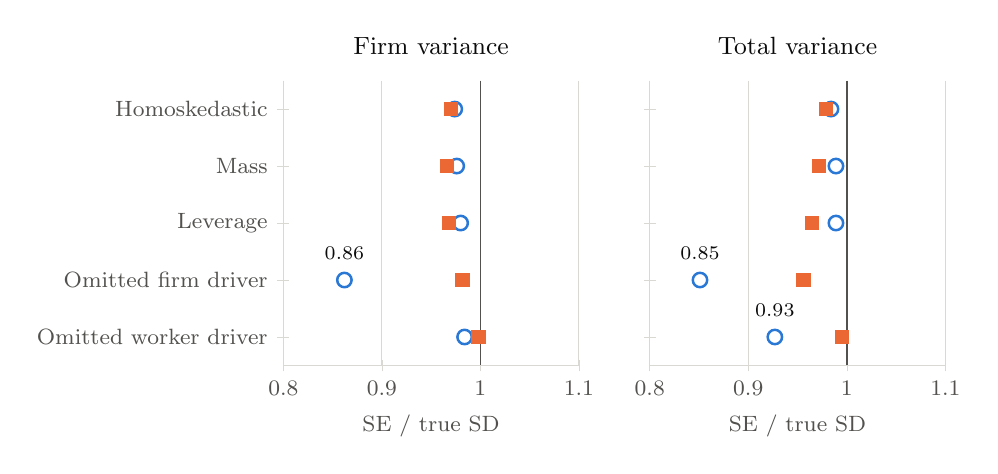
\begin{tikzpicture}
\begin{groupplot}[
  group style={group size=2 by 1, horizontal sep=0.9cm, y descriptions at=edge left},
  width=0.44\linewidth, height=5.2cm,
  xmin=0.80, xmax=1.10, xtick={0.8,0.9,1.0,1.1},
  ymin=0.5, ymax=5.5, y dir=reverse,
  ytick={1,2,3,4,5},
  yticklabels={Homoskedastic, Mass, Leverage, Omitted firm driver, Omitted worker driver},
  tick label style={font=\footnotesize, color=inkmuted},
  title style={font=\small, color=ink},
  xlabel style={font=\footnotesize, color=inkmuted},
  tick style={gridline},
  xmajorgrids, grid style={gridline, line width=0.3pt},
  axis lines=left, axis line style={gridline, -}, clip=false,
]
\nextgroupplot[title={Firm variance}, xlabel={SE / true SD},
  legend to name=mainlegend,
  legend style={font=\footnotesize, draw=none, legend columns=2, column sep=1em, text=ink}]
\draw[inkmuted, line width=0.6pt] (axis cs:1,0.5) -- (axis cs:1,5.5);
\addplot[only marks, mark=o, mark size=2.6pt, line width=0.9pt, seriesA]
  coordinates {(0.974,1) (0.976,2) (0.980,3) (0.862,4) (0.984,5)};
\addlegendentry{Model-based}
\addplot[only marks, mark=square*, mark size=2.4pt, seriesB]
  coordinates {(0.970,1) (0.966,2) (0.968,3) (0.982,4) (0.998,5)};
\addlegendentry{Reported}
\node[font=\scriptsize, color=ink, anchor=south] at (axis cs:0.862,3.82) {0.86};
\nextgroupplot[title={Total variance}, xlabel={SE / true SD}]
\draw[inkmuted, line width=0.6pt] (axis cs:1,0.5) -- (axis cs:1,5.5);
\addplot[only marks, mark=o, mark size=2.6pt, line width=0.9pt, seriesA]
  coordinates {(0.984,1) (0.989,2) (0.989,3) (0.851,4) (0.927,5)};
\addplot[only marks, mark=square*, mark size=2.4pt, seriesB]
  coordinates {(0.979,1) (0.972,2) (0.965,3) (0.956,4) (0.995,5)};
\node[font=\scriptsize, color=ink, anchor=south] at (axis cs:0.851,3.82) {0.85};
\node[font=\scriptsize, color=ink, anchor=south] at (axis cs:0.927,4.82) {0.93};
\end{groupplot}
\end{tikzpicture}

\smallskip
\pgfplotslegendfromname{mainlegend}
\caption{Standard error relative to the true sampling standard deviation,
from Table~\ref{tab:main}. The vertical line marks a correct standard error.
When the variance model is adequate the two methods agree. When a variance
driver is omitted, the model-based standard error is up to 15\% too small and
the reported one stays within 5\%.}\label{fig:main}
\end{figure}

Three further results from the same design:
\begin{itemize}
\item Fitting the working variances from leave-out products
\eqref{eq:working}, with no solve, gives the same model-based standard
errors as the residual-moment fit, to within 0.012 in the SE ratio in every
design.
\item With a homoskedastic working model the reported SE ratios are 0.96 to
1.06 across the five designs, so the method leans little on the working
model. That crude model does fail for a firm variance close to zero (0.91
before truncation), which is why the small leverage-and-mass model is the
default.
\item Two other designs give the same picture. With 57\% of units being
stayer observations (4,650 units, 800 samples) the reported SE ratios are
0.96 to 1.07 and coverage is 0.927 to 0.963, against 0.83 to 0.87 for the
model-based firm and total standard errors under the omitted firm driver.
With movers only and less mobility (4,148 units, 6.5 matches per firm, mean
leverage 0.59) they are 0.96 to 1.10 with coverage 0.940 to 0.968.
\end{itemize}

\subsection{Controls and deletion units}

Table~\ref{tab:controls} uses a physical-row version of the prototype
(3,350 observations, 627 workers, 130 firms). The truth is the exact variance
of the \emph{jointly} estimated leave-unit-out estimator, computed from its
dense block kernel. The standard error is always computed on collapsed units
with the fitted offset. Controls vary within units and are correlated with
firm type.

\begin{table}[ht]
\centering\small
\begin{tabular}{@{}llcccc@{\hskip 1.2em}c@{\hskip 1.2em}c@{}}
\toprule
 & & \multicolumn{4}{c}{SE ratio, with control term} & Total, & Coverage, \\
Deletion, controls & Errors & wkr & firm & cov & total & without & with \\
\midrule
Match, none & base & 0.989 & 0.995 & 1.006 & 0.984 & -- & .934--.956 \\
Match, none & omitted firm & 1.064 & 0.988 & 0.978 & 0.973 & -- & .930--.960 \\
Match, 2 & base & 0.972 & 0.993 & 0.992 & 0.989 & 0.787 & .938--.952 \\
Match, 2 & omitted firm & 1.046 & 0.987 & 0.972 & 0.984 & 0.785 & .926--.958 \\
Match, 2 & omitted worker & 1.020 & 1.017 & 1.031 & 1.016 & 0.840 & .946--.954 \\
Match, 6 & base & 0.969 & 0.991 & 0.991 & 0.987 & 0.785 & .938--.950 \\
Declared parts of matches, 2 & base & 0.995 & 0.995 & 0.989 & 0.990 & 0.709 & .942--.954 \\
Declared parts of matches, 2 & omitted firm & 1.019 & 0.992 & 0.980 & 0.980 & 0.715 & .926--.956 \\
Observation, 2 & base & 0.999 & 1.001 & 0.997 & 1.000 & 0.692 & .942--.952 \\
Observation, 2 & omitted firm & 1.016 & 0.999 & 0.993 & 0.993 & 0.698 & .936--.944 \\
\bottomrule
\end{tabular}
\caption{Controls and deletion units, 500 samples per row. SE ratios are
against the exact standard deviation of the jointly estimated estimator.
``Total, without'' is the SE ratio for the total when the control term
\eqref{eq:score} is left out. Coverage is the range over the four components
for the jointly estimated estimate. Base errors have a unit-level random
effect under match deletion and are independent under observation deletion.}
\label{tab:controls}
\end{table}

The fixed-offset estimate has the same coverage as the joint one to within
0.01 in every row. A second design seed with two controls gives SE ratios of
0.985 to 1.034. The corrected-centering adjustment has a root-mean-square
size of 0.0002 to 0.0009 standard deviations, and the corrected estimate has
the same coverage as the mean-centred one.

\subsection{Random-projection leverages and scale}

Table~\ref{tab:scale} runs the matrix-free calculation with leverages and
target diagonals from 200 Rademacher probes and $R=8$ draws, 36 solves in the
second pass including the fit. SE ratios are against the analytic standard
deviation of the estimate, computed from its kernel and the true variances.

\begin{table}[ht]
\centering\small
\begin{tabular}{@{}rlcccc@{\hskip 1.2em}cccc@{}}
\toprule
 & & \multicolumn{4}{c}{Reported SE ratio} & \multicolumn{4}{c}{Model-based SE ratio} \\
Units & Errors & wkr & firm & cov & total & wkr & firm & cov & total \\
\midrule
4,413 & mass & 0.990 & 0.983 & 0.973 & 0.977 & 1.001 & 1.000 & 1.008 & 0.997 \\
4,413 & omitted firm & 1.063 & 0.982 & 0.973 & 0.957 & 1.007 & 0.869 & 0.913 & 0.857 \\
56,486 & homoskedastic & 1.002 & 1.002 & 0.998 & 1.001 & 1.000 & 1.000 & 1.005 & 1.000 \\
56,486 & mass & 1.002 & 0.996 & 0.973 & 0.992 & 1.000 & 0.999 & 1.004 & 0.999 \\
56,486 & omitted firm & 1.108 & 0.989 & 1.010 & 0.945 & 1.045 & 0.944 & 0.880 & 0.817 \\
56,486 & omitted worker & 1.021 & 1.007 & 1.020 & 1.014 & 0.983 & 1.002 & 0.965 & 0.933 \\
358,809 & mass & 1.006 & 1.001 & 0.972 & 0.996 & 1.006 & 0.998 & 1.007 & 1.000 \\
358,809 & omitted firm & 1.107 & 0.989 & 1.003 & 0.957 & 1.044 & 0.937 & 0.848 & 0.808 \\
\bottomrule
\end{tabular}
\caption{Matrix-free calculation. 500 samples at 4,413 units, 120 at 56,486,
one outcome at 358,809. Here ``model-based'' uses the working variances of
\eqref{eq:working} in the signal term.}\label{tab:scale}
\end{table}

Coverage of the reported interval is 0.930 to 0.976 at 4,413 units and 0.917
to 0.967 at 56,486, where 120 samples give a Monte Carlo standard error of
0.02. All variances are positive after truncation; before it, the covariance
component's variance was negative in 0.2 to 0.4\% of samples at 4,413 units.

\paragraph{How many draws.} For one outcome at 4,413 units, the coefficient
of variation of the reported standard error across pseudo-noise seeds is 1.5
to 5.0\% with two draws, 0.8 to 3.5\% with eight and 0.5 to 1.7\% with
sixteen; the larger figure is always the covariance component. At 358,809
units it is at most 0.35\% with two draws and 0.07\% with eight. One draw
estimates the trace with a coefficient of variation of 4 to 10\% at 4,413
units, against 19 to 21\% for fifty solves of the scalar estimator. Eight
draws give $\reff$ of 1,184, 392 and 230 against exact values of 1,209, 346
and 198.

\subsection{Stress cases}

\begin{table}[ht]
\centering\small
\begin{tabular}{@{}lcccc@{\hskip 1.2em}cccc@{}}
\toprule
 & \multicolumn{4}{c}{SE ratio} & \multicolumn{4}{c}{Coverage} \\
Case & wkr & firm & cov & total & wkr & firm & cov & total \\
\midrule
Weak firm variance, mass errors & 0.979 & 0.981 & 1.009 & 0.970 & .942 & .942 & .953 & .948 \\
Weak firm variance, omitted firm driver & 1.055 & 1.063 & 1.005 & 0.998 & .961 & .958 & .952 & .951 \\
Very weak firm variance, mass errors & 0.978 & 0.983 & 1.005 & 0.971 & .941 & .944 & .951 & .948 \\
Skewed errors, omitted firm driver & 1.130 & 0.974 & 1.048 & 1.005 & .971 & .936 & .955 & .955 \\
$t_5$ errors, mass & 1.136 & 1.031 & 1.049 & 1.115 & .962 & .945 & .952 & .960 \\
$t_5$ errors, omitted firm driver & 1.273 & 1.030 & 1.087 & 1.118 & .976 & .949 & .951 & .953 \\
\bottomrule
\end{tabular}
\caption{Stress cases, 4,413 units, 1,000 samples. The standard deviation of
the firm-variance estimate is 33 to 39\% of the component in the weak cases
and 70\% in the very weak case. Skewed errors are centred chi-square with
three degrees of freedom.}\label{tab:stress}
\end{table}

A variance was available in every sample. For the weak firm variance the
truncation in \eqref{eq:final} raises coverage from 0.92--0.93 to 0.94. Under
$t_5$ errors the median SE ratio is 0.99 to 1.14; the root-mean-square
figures in Table~\ref{tab:stress} are inflated by the heavy tail of the
variance estimate itself.

\paragraph{A dominant direction.} With two groups of firms joined by twelve
movers the exact leading shares are 0.79 to 0.90. Normal intervals then
under-cover for every method, including one that uses the true variances
(0.89 for the firm variance and 0.85 for the covariance). Sixteen draws
estimate $\reff$ as 1.6, 1.3 and 1.2, equal to the exact values, and eight
draws give 3.4, 1.9 and 1.8, against hundreds or thousands in the other
designs. The diagnostic separates the two situations clearly.

\subsection{What this evidence does not establish}

The prototype is written in Python with a direct sparse factorisation. It
uses a plain reciprocal for the residual-maker inverse where \fevc{} uses a
finite-projection formula, and Gaussian errors unless stated. Designs are
synthetic, the largest Monte Carlo design has 56,486 units, and nothing was
pre-registered. Controls appear only in the dense physical-row harness. The
evidence supports the algebra and the design choice; it is not a
qualification of the released command.

\section{Implementation status}\label{sec:status}

\begin{sloppypar}
This section records what exists in the repository at the time of
writing, and how each part was checked. Stata was not available where this
work was done, so no Stata or Mata code described here has been executed.

\paragraph{Default behaviour.} Standard errors are requested by default
(\texttt{inference(auto)}). The command computes them whenever the request
can carry them and otherwise returns point estimates with a stated reason. It
never changes the backend, algorithm or solver route the user selected. If
the native executor or the Mata stage that carries them stops, the command
runs once more without them, so the point estimates do not depend on the
standard errors; option, variable and sample errors are reported once.
\texttt{inference(none)} gives point estimates only, and
\texttt{inferencemodel(leaveout\_residual)} with \texttt{inference(highrank)}
requests the standard errors strictly.

\paragraph{Rust core and plugin (tested).} The method is implemented in
\texttt{rust/\allowbreak crates/\allowbreak vckss-core/\allowbreak src/\allowbreak residual\_noise.rs} and attached to the
generic JLA engine. It covers observation units with controls kept in the
operator and collapsed deletion units under either nuisance mode, with
pooled stayers, frequency weights for match deletion, the automatic solver
route, both of the plugin's automatic executors, numerical MCSE replay and
all three centering modes. Tests compare the kernel image of the outcome, the
pseudo-noise moments, the control term and the assembled covariance with
independent dense calculations, and end-to-end tests drive the plugin's C
interface through the entry points the default command uses. The public
interface reports the method as variance source 3 behind a capability flag;
the plugin binaries shipped in the repository predate it and must be rebuilt
before Stata can use it. Until then the default returns point estimates and
says so.

\paragraph{Controls kept in the operator.} Under the default
\texttt{nuisance(joint)} with match deletion, the engine forms the
fixed-offset unit geometry beside the joint point estimate. The leverage
moments are shared, the leave-out adjustments are recomputed without controls
at no solve cost, and one further target pass uses the worker--firm solver on
the offset outcome: two solves per probe, 400 by default. The point estimate
is unchanged, and the standard errors equal those of a fixed-offset run to
solver tolerance.

\paragraph{Engine selection.} The compressed engine serves requests with
match deletion, no controls and no stayers. It carries no attachment, so such
a request runs on the generic engine when standard errors are computed, as
the same request already does whenever stayers or controls are present. The
two engines estimate the same quantities.

\paragraph{Mata (written, not executed).}
\texttt{fevc\_residual\_se.mata} is loaded only when standard errors are
computed on the Mata backend, so it cannot affect other estimates. It holds
two routines. The first uses exact kernels for \texttt{algorithm(exact)} with
match deletion. The second is matrix-free and serves \texttt{algorithm(jla)}
and observation deletion: it is a separate stage that draws its own
projections, forms the residual-maker inverse with the finite-projection
correction the point estimator uses, and costs about three solves per probe,
one per control and four per draw, roughly as much as the point estimates.
Statement-by-statement numpy transliterations of both routines reproduce the
dense oracle (\texttt{check\_mata\_mirror.py}): for the exact routine every
intermediate quantity to $10^{-13}$ and standard errors within 0.2\% of
closed form; for the matrix-free routine, at 200 probes and 8 draws, standard
errors within 3.5\% of the exact sampling standard deviation of the jointly
estimated estimator, for match and observation deletion with zero, two and
six controls. That checks the algorithms, not the Mata syntax.

\paragraph{Stata front end (written, not executed).} The route validation,
attachment, receipt reconciliation, posting, display and help were changed
for the new default. A regression file,
\texttt{tests/stata/test\_leaveout\_residual\_se.do}, exercises the default
request and its routes and is likewise unexecuted. The registered suites
were written for the point-only default; the environment setting
\texttt{FEVC\_DEFAULT\_INFERENCE=none} keeps them on it.

\paragraph{Not covered.} The default returns point estimates, with a reason,
for \texttt{project()} in the same call, for observation deletion with a
fixed offset or, on the native backend, with frequency weights, for
\texttt{algorithm(auto)}, and for \texttt{algorithm(exact)} on the native
backend. Two smaller items remain. The memory forecast of the attachment
reuses the formula of the structured sources; its allowances exceed this
method's buffers, but it was not re-derived for them. The model-based
covariance and the working-variance term counts are in the core result but
not yet in the Stata transport.
\end{sloppypar}

\appendix
\section{Derivations}\label{sec:derivations}

\paragraph{The residual statistic.} Write $g_{ta}=m_{ta}+n_{ta}$ with
$n_t=K_t\varepsilon$, and $e=M\varepsilon$. Then
\[
 \E[g_{ta}g_{sa}e_a^2]=m_{ta}m_{sa}\E[e_a^2]
 +m_{ta}\E[n_{sa}e_a^2]+m_{sa}\E[n_{ta}e_a^2]+\E[n_{ta}n_{sa}e_a^2].
\]
Here $\E[e_a^2]=(MVM)_{aa}=M_{aa}^2\sigma_a^2+\sum_{b\ne a}P_{ab}^2\sigma_b^2$.
Dividing by $M_{aa}$ and using $\sum_{b\neq a}P_{ab}^2=P_{aa}M_{aa}$ gives
\eqref{eq:sigmabar}. The middle terms are third cumulants,
$\sum_bK_{tab}M_{ab}^2\kappa_{3,b}$, and vanish for symmetric errors. For
Gaussian errors the last term is
$(K_tVK_s)_{aa}(MVM)_{aa}+2(K_tVM)_{aa}(K_sVM)_{aa}$, which is the summand of
\eqref{eq:noise}; other error laws add
$\sum_bK_{tab}K_{sab}M_{ab}^2\kappa_{4,b}$, which is non-negative for $t=s$
when $\kappa_{4,b}\ge0$.

\paragraph{The trace estimate.} For $\zeta=\tilde V^{1/2}\xi$ with standard
normal $\xi$, $\sum_a\tilde\sigma_a^2(K_t\zeta)_a^2=\xi'W_t^2\xi$, whose mean
is $\tr(W_t^2)=\tr(K_t\tilde VK_t\tilde V)$ and whose variance is
$2\tr(W_t^4)$. Its squared coefficient of variation is therefore $2/\reff$.
For independent $\xi,\xi'$, $\E(\xi'W_t^2\xi')^2=\tr(W_t^4)$, which gives the
pair estimate of $\reff$. The bracket \eqref{eq:bracket} follows from
$\lambda_1^4\le\sum_j\lambda_j^4\le\lambda_1^2\sum_j\lambda_j^2$.

\paragraph{Joint and fixed-offset estimates.} Both use the same two-way
coefficients, because the joint fit of the effects equals their fit to
$y-Z\hat\gamma$. They differ in the leave-out correction, where the joint
version also lets $\gamma$ move; that difference is of order $k/n$ relative
to the correction for $k$ controls. Projecting the full design gives
$P_{[D,Z]}=P_D+\tilde Z\Lambda\tilde Z'$, so $\hat\gamma-\gamma=
\Lambda\tilde Z'\varepsilon$, and a first-order expansion of the fixed-offset
estimate in $\gamma$ gives \eqref{eq:score}. Within a unit,
$\sum_{i\in a}\tilde z_i\varepsilon_i$ splits into the product of unit
aggregates, estimated with the HC2-scaled unit residual, and the within-unit
cross-product $w_a$, in which residual deviations equal outcome deviations.

\paragraph{Corrected centering on collapsed units.} With $s_a$ the leave-out
product, $F_a$ the unit mass, $n=\sum_aF_a$ and
$D_F=\diag(\sqrt{F_a})$, the documented adjustment is
$\Delta_t=-\sum_aB_{t,aa}\kappa_a$ with
$\kappa=D_F^{-1}\{n\,\diag(M_{aa}/F_a)-M\}^{-1}MD_Fs$.

\section*{References}
\begin{description}[leftmargin=1.5em,labelindent=0em,itemsep=2pt]
\item Cattaneo, M. D., M. Jansson and W. K. Newey (2018). Inference in linear
regression models with many covariates and heteroscedasticity. \emph{Journal
of the American Statistical Association} 113, 1350--1361.
\item Hutchinson, M. F. (1990). A stochastic estimator of the trace of the
influence matrix for Laplacian smoothing splines. \emph{Communications in
Statistics -- Simulation and Computation} 19, 433--450.
\item Kline, P., R. Saggio and M. S{\o}lvsten (2020). Leave-out estimation of
variance components. \emph{Econometrica} 88, 1859--1898.
\item MacKinnon, J. G. and H. White (1985). Some heteroskedasticity-consistent
covariance matrix estimators with improved finite sample properties.
\emph{Journal of Econometrics} 29, 305--325.
\end{description}

\end{document}
